% =============================================================================
%  Diplomado en Data Science Aplicada con Python para la Toma de Decisiones
%  Clase 37: Agentes — el analista que programa por ti
%  Arca Continental Ecuador | UDLA
% =============================================================================
\documentclass[aspectratio=169, 11pt]{beamer}

\usepackage[T1]{fontenc}
\usepackage[utf8]{inputenc}
\usepackage[spanish,es-noshorthands]{babel}
\usepackage{FiraSans}
\usepackage{FiraMono}
\renewcommand{\familydefault}{\sfdefault}
\usepackage{graphicx}
\usepackage{tikz}
\usetikzlibrary{arrows.meta, positioning, shapes.geometric, shapes.misc,
  calc, fit, decorations.pathreplacing, backgrounds, matrix, chains}
\usepackage{fontawesome5}
\usepackage{minted}
\usepackage{tcolorbox}
\tcbuselibrary{minted, skins, breakable}
\usepackage{booktabs}
\usepackage{multicol}
\usepackage{hyperref}
\usepackage{calc}
\usepackage{amsmath}

\definecolor{arcaRed}{HTML}{C82B40}
\definecolor{arcaDark}{HTML}{6B1525}
\definecolor{arcaGray}{HTML}{F5F5F5}
\definecolor{arcaLightGray}{HTML}{EBEBEB}
\definecolor{textDark}{HTML}{2D2D2D}
\definecolor{textMuted}{HTML}{6B7280}
\definecolor{codeGreen}{HTML}{16A34A}
\definecolor{codeBlue}{HTML}{2563EB}
\definecolor{codeOrange}{HTML}{EA580C}
\definecolor{codePurple}{HTML}{7C3AED}

\usetheme{default}
\usecolortheme{default}
\setbeamertemplate{navigation symbols}{}
\setbeamertemplate{footline}{}
\setbeamertemplate{headline}{}
\setbeamercolor{normal text}{fg=textDark}
\setbeamercolor{frametitle}{fg=arcaRed, bg=white}
\setbeamercolor{title}{fg=white}
\setbeamercolor{subtitle}{fg=white!85}
\setbeamercolor{author}{fg=white!80}
\setbeamercolor{date}{fg=white!70}
\setbeamercolor{item}{fg=arcaRed}
\setbeamercolor{subitem}{fg=arcaDark}
\setbeamerfont{frametitle}{size=\Large, series=\bfseries}
\setbeamerfont{title}{size=\huge, series=\bfseries}
\setbeamerfont{subtitle}{size=\large}
\setbeamertemplate{itemize item}{\scriptsize\raise1.5pt\hbox{\color{arcaRed}$\blacktriangleright$}}
\setbeamertemplate{itemize subitem}{\scriptsize\raise1pt\hbox{\color{arcaDark}$\bullet$}}
\setbeamertemplate{enumerate items}[default]
\setbeamercolor{enumerate item}{fg=arcaRed}

\setbeamertemplate{headline}{%
  \begin{tikzpicture}[remember picture, overlay]
    \fill[arcaDark] (current page.north west) rectangle
      ([yshift=-0.7cm]current page.north east);
    \node[anchor=west, inner sep=0pt] at
      ([xshift=0.6cm, yshift=-0.35cm]current page.north west)
      {
\includegraphics[height=0.45cm]{../logo_udla_white.png}};
    \node[anchor=east, inner sep=0pt] at
      ([xshift=-0.6cm, yshift=-0.35cm]current page.north east)
      {
\includegraphics[height=0.45cm]{../ArcaContinental_white.png}};
  \end{tikzpicture}%
  \vspace{0.7cm}%
}

\setbeamertemplate{footline}{%
  \begin{tikzpicture}[remember picture, overlay]
    \node[anchor=south east, font=\scriptsize\bfseries\color{arcaRed}] at
      ([xshift=-0.5cm, yshift=0.15cm]current page.south east)
      {\insertframenumber};
  \end{tikzpicture}%
  \vspace{0.3cm}%
}

\setbeamertemplate{frametitle}{%
  \vspace{0.25cm}%
  \usebeamerfont{frametitle}\usebeamercolor[fg]{frametitle}\insertframetitle%
  \par\vspace{2pt}%
  \begin{tikzpicture}
    \fill[arcaRed] (0,0) rectangle (3cm, 1.5pt);
    \fill[arcaLightGray] (3cm,0) rectangle (\textwidth, 0.5pt);
  \end{tikzpicture}%
  \vspace{0.1cm}%
}

\newtcblisting{pyblock}[1][]{%
  listing engine=minted, minted language=python, minted style=friendly,
  minted options={fontsize=\small, linenos=false, breaklines=true, python3=true},
  colback=arcaGray, colframe=arcaRed, left=4pt, right=4pt, top=4pt, bottom=4pt,
  boxrule=0pt, leftrule=3pt, arc=2pt, listing only, #1}

\newcommand{\sectionframe}[2]{%
  \begingroup
  \setbeamertemplate{headline}{}%
  \setbeamertemplate{footline}{}%
  \begin{frame}[plain, noframenumbering]
    \begin{tikzpicture}[remember picture, overlay]
      \fill[arcaRed] (current page.south west) rectangle (current page.north east);
      \node[anchor=center, text=white, font=\Huge\bfseries, text width=12cm,
            align=center] at ([yshift=0.5cm]current page.center) {#1};
      \node[anchor=center, text=white!80, font=\large, text width=11cm,
            align=center] at ([yshift=-0.9cm]current page.center) {#2};
    \end{tikzpicture}
  \end{frame}
  \endgroup
}

\tikzset{
  arrowR/.style={-{Stealth[length=2.5mm]}, arcaRed, thick},
  arrowD/.style={-{Stealth[length=2.5mm]}, arcaDark, thick},
  arrowG/.style={-{Stealth[length=2.5mm]}, color=textMuted, thick, dashed},
  boxA/.style={rectangle, rounded corners=4pt, draw=arcaDark, fill=arcaGray,
               align=center, font=\footnotesize, inner sep=4pt, minimum height=0.9cm},
  boxRed/.style={rectangle, rounded corners=4pt, draw=arcaDark, fill=arcaRed,
                 text=white, align=center, font=\bfseries\footnotesize,
                 inner sep=5pt, minimum height=0.9cm},
  boxBlue/.style={rectangle, rounded corners=4pt, draw=arcaDark, fill=codeBlue,
                  text=white, align=center, font=\bfseries\footnotesize,
                  inner sep=5pt, minimum height=0.9cm},
  boxGreen/.style={rectangle, rounded corners=4pt, draw=arcaDark, fill=codeGreen,
                   text=white, align=center, font=\bfseries\footnotesize,
                   inner sep=5pt, minimum height=0.9cm},
  boxOrange/.style={rectangle, rounded corners=4pt, draw=arcaDark, fill=codeOrange,
                    text=white, align=center, font=\bfseries\footnotesize,
                    inner sep=5pt, minimum height=0.9cm},
  boxPurple/.style={rectangle, rounded corners=4pt, draw=arcaDark, fill=codePurple,
                    text=white, align=center, font=\bfseries\footnotesize,
                    inner sep=5pt, minimum height=0.9cm},
}

\newtcolorbox{idea}{colback=arcaRed!8, colframe=arcaRed, leftrule=3pt,
  boxrule=0pt, sharp corners, left=8pt, right=8pt, top=6pt, bottom=6pt}
\newtcolorbox{nota}{colback=arcaGray, colframe=arcaDark, leftrule=3pt,
  boxrule=0pt, sharp corners, left=8pt, right=8pt, top=6pt, bottom=6pt}

\title{Diplomado en Data Science Aplicada\\con Python para la Toma de Decisiones}
\subtitle{Clase 37: Agentes --- el analista que programa por ti}
\author{Carlos Enrique Mosquera Trujillo}
\date{11 de Junio, 2026}

\begin{document}

% =====================================================================
%  PORTADA
% =====================================================================
{
\setbeamertemplate{headline}{}
\setbeamertemplate{footline}{}
\begin{frame}[plain, noframenumbering]
  \begin{tikzpicture}[remember picture, overlay]
    \fill[arcaDark] (current page.south west) rectangle (current page.north east);
    \fill[arcaRed] ([yshift=-3.5cm]current page.north west) rectangle
      ([yshift=-4.2cm]current page.north east);
    \node[anchor=west, inner sep=0pt] at
      ([xshift=1cm, yshift=-1.5cm]current page.north west)
      {
\includegraphics[height=1cm]{../logo_udla_white.png}};
    \node[anchor=east, inner sep=0pt] at
      ([xshift=-1cm, yshift=-1.5cm]current page.north east)
      {
\includegraphics[height=1cm]{../ArcaContinental_white.png}};
  \end{tikzpicture}
  \vspace{2.5cm}
  \begin{center}
    {\usebeamerfont{title}\usebeamercolor[fg]{title}\inserttitle\par}
    \vspace{0.4cm}
    {\usebeamerfont{subtitle}\usebeamercolor[fg]{subtitle}\insertsubtitle\par}
    \vspace{0.6cm}
    {\usebeamerfont{author}\usebeamercolor[fg]{author}\insertauthor\par}
    \vspace{0.15cm}
    {\usebeamerfont{date}\usebeamercolor[fg]{date}\insertdate\par}
  \end{center}
\end{frame}
}

% =====================================================================
%  BLOQUE 0
% =====================================================================
\sectionframe{Bloque 0}{De un modelo que \emph{habla}\\a un agente que \emph{actúa}}

% F2 — recap + pregunta del dia
\begin{frame}{De dónde venimos, a dónde vamos}
  \vspace{8pt}
  \begin{nota}{\small\color{arcaDark}
    En la clase 36 (bonus) armamos un agente \textbf{a mano}: escribimos el bucle,
    definimos la herramienta, parseamos el JSON del modelo. Funcionó, pero fue mucho
    código y muy frágil.}
  \end{nota}
  \vspace{14pt}
  \begin{idea}{\small\color{arcaDark}\bfseries
    Pregunta del día: ¿y si en vez de programar el análisis, le \textbf{hablamos en
    español} a un agente y \textbf{él escribe y ejecuta el código} por nosotros?}
  \end{idea}
  \vspace{10pt}
  \begin{center}{\footnotesize\color{textMuted}
  Hoy: tu trabajo es \emph{preguntar bien}; el trabajo del agente es \emph{programar}.}\end{center}
\end{frame}

% =====================================================================
%  BLOQUE 1 — Qué es / historia / mercado
% =====================================================================
\sectionframe{Bloque 1}{¿Qué es un agente?\\Historia y por qué importa}

% F3 — chatbot vs agente
\begin{frame}{Chatbot vs. agente}
  \vspace{2pt}
  \begin{center}
  \begin{tikzpicture}[font=\footnotesize, node distance=0.45cm and 1.2cm]
    \node[boxA, minimum width=3.0cm] (c1) {pregunta};
    \node[boxRed, right=of c1, minimum width=2.2cm] (c2) {LLM};
    \node[boxA, right=of c2, minimum width=3.0cm] (c3) {responde};
    \draw[arrowR] (c1)--(c2); \draw[arrowR] (c2)--(c3);
    \node[left=0.2cm of c1, text=textMuted, font=\bfseries\scriptsize] {CHATBOT};
    \node[boxA, below=1.0cm of c1, minimum width=3.0cm] (a1) {objetivo};
    \node[boxRed, right=of a1, minimum width=2.2cm] (a2) {LLM};
    \node[boxBlue, right=of a2, minimum width=3.0cm, align=center] (a3) {actúa\\(usa código/tools)};
    \node[fill=arcaDark, text=white, rounded corners=4pt, right=1.2cm of a3,
          font=\bfseries\scriptsize, inner sep=5pt, align=center] (a4) {logra\\la tarea};
    \draw[arrowR] (a1)--(a2); \draw[arrowR] (a2)--(a3); \draw[arrowR] (a3)--(a4);
    \draw[arrowG] (a3.south) .. controls +(0,-0.7) and +(0,-0.7) .. (a2.south);
    \node[left=0.2cm of a1, text=arcaRed, font=\bfseries\scriptsize] {AGENTE};
  \end{tikzpicture}
  \end{center}
  \vspace{6pt}
  \begin{idea}{\small\color{arcaDark}\bfseries
    El chatbot \emph{responde}. El agente \emph{decide, actúa y repite} hasta lograr un objetivo.}
  \end{idea}
\end{frame}

% F4 — el bucle ReAct
\begin{frame}{El bucle ReAct: pensar $\to$ actuar $\to$ observar}
  \vspace{8pt}
  \begin{center}
  \begin{tikzpicture}[font=\scriptsize, node distance=0.45cm and 0.7cm]
    \node[boxA, minimum width=2.1cm] (q) {pedido};
    \node[boxRed, right=of q, minimum width=2.2cm, align=center] (p) {1. Piensa\\(plan)};
    \node[boxBlue, right=of p, minimum width=2.2cm, align=center] (a) {2. Actúa\\(escribe código)};
    \node[boxGreen, right=of a, minimum width=2.2cm, align=center] (o) {3. Observa\\(ejecuta)};
    \node[fill=arcaDark, text=white, rounded corners=4pt, right=of o,
          font=\bfseries\scriptsize, inner sep=5pt] (ans) {responde};
    \draw[arrowR] (q)--(p); \draw[arrowR] (p)--(a); \draw[arrowR] (a)--(o); \draw[arrowR] (o)--(ans);
    \draw[arrowG] (o.south) .. controls +(0,-0.8) and +(0,-0.8) .. (p.south)
      node[midway, below, font=\scriptsize\itshape] {¿falta? repite};
  \end{tikzpicture}
  \end{center}
  \vspace{12pt}
  \begin{nota}{\small\color{arcaDark}
    Publicado en 2022 (\emph{ReAct}, Princeton + Google). Intercalar razonamiento y
    acción mejoró tareas complejas hasta \textbf{+34\%} frente a responder de una sola vez.
    Es la base de casi todos los agentes de hoy.}
  \end{nota}
\end{frame}

% F5 — timeline
\begin{frame}{¿Por qué AHORA? La línea de tiempo}
  \vspace{6pt}
  \begin{center}
  \begin{tikzpicture}[font=\scriptsize]
    \draw[arcaLightGray, line width=3pt] (0,0) -- (12.2,0);
    \foreach \x in {0.7, 4.4, 7.7, 11.3} \fill[arcaRed] (\x,0) circle (3pt);
    \node[boxRed, anchor=south] at (0.7,0.35) {2022};
    \node[boxBlue, anchor=south] at (4.4,0.35) {2023};
    \node[boxBlue, anchor=south] at (7.7,0.35) {2023};
    \node[boxOrange, anchor=south] at (11.3,0.35) {2024};
    \node[anchor=north, text width=2.4cm, align=center] at (0.7,-0.3)
      {\textbf{ReAct}\\razonar + actuar};
    \node[anchor=north, text width=2.7cm, align=center] at (4.4,-0.3)
      {\textbf{Function calling}\\el modelo pide funciones};
    \node[anchor=north, text width=2.4cm, align=center] at (7.7,-0.3)
      {\textbf{AutoGPT}\\la explosión};
    \node[anchor=north, text width=2.4cm, align=center] at (11.3,-0.3)
      {\textbf{MCP}\\estándar de conexión};
  \end{tikzpicture}
  \end{center}
  \vspace{16pt}
  \begin{nota}{\footnotesize\color{arcaDark}
    El desbloqueo fue el \textbf{function calling} (OpenAI/Google, 2023): el modelo emite
    un JSON pidiendo una acción de forma fiable. \textbf{MCP} (Anthropic, 2024) estandarizó
    cómo conectar agentes con herramientas; lo adoptaron OpenAI y Google.}
  \end{nota}
\end{frame}

% F6 — mercado
\begin{frame}{¿Por qué es un negocio multimillonario?}
  \vspace{10pt}
  \begin{center}
  \begin{tikzpicture}[font=\footnotesize, node distance=0.9cm]
    \node[boxRed, text width=2.9cm, minimum height=1.5cm]
      (a) {\Large \$7.8\,B\\[2pt]\scriptsize mercado 2025};
    \node[boxOrange, right=of a, text width=2.9cm, minimum height=1.5cm]
      (b) {\Large \$52\,B\\[2pt]\scriptsize proyección 2030};
    \node[boxBlue, right=of b, text width=2.9cm, minimum height=1.5cm]
      (c) {\Large 40\%\\[2pt]\scriptsize apps con agentes (2026)};
    \draw[arrowD] (a)--(b);
  \end{tikzpicture}
  \end{center}
  \vspace{12pt}
  \begin{nota}{\footnotesize\color{arcaDark}
    Crecimiento $\sim$46\% anual. Gartner: del \textbf{$<$5\% (2025) al 40\% (2026)} de
    apps empresariales con agentes; hacia 2035 podrían ser $\sim$\$450\,B.
    No pagan por "chatear": pagan por \textbf{automatizar trabajo}.
    \hfill{\scriptsize\color{textMuted}Fuentes: MarketsandMarkets, Gartner.}}
  \end{nota}
\end{frame}

% F7 — casos + anti-hype
\begin{frame}{Casos reales --- y la letra chica}
  \vspace{4pt}
  {\footnotesize
  \begin{tabular}{@{}p{2.7cm}p{9.3cm}@{}}
    \textbf{Klarna} & 1 agente de atención $\approx$ 853 personas; resolución 11 min $\to$ \textbf{$<$2 min}.\\[2pt]
    \textbf{Morgan Stanley} & revisó \textbf{9M} de líneas de código; $\sim$280.000 horas ahorradas.\\[2pt]
    \textbf{DoorDash} & agente de voz: cientos de miles de llamadas/día.\\
  \end{tabular}}
  \vspace{8pt}
  \begin{idea}{\footnotesize\color{arcaDark}\bfseries
    Anti-hype (honestidad): \textbf{79\%} dicen haberlos adoptado, pero solo \textbf{11\%}
    están en producción; Gartner estima que \textbf{40\%} de los proyectos se cancelarán
    para 2027 (costo, valor poco claro). Del demo a producción hay un trecho.}
  \end{idea}
\end{frame}

% =====================================================================
%  BLOQUE 2 — CodeAgent
% =====================================================================
\sectionframe{Bloque 2}{El CodeAgent:\\le hablas, él programa}

% F8 — dos familias
\begin{frame}{Dos familias de agentes}
  \vspace{8pt}
  {\footnotesize
  \begin{tabular}{@{}p{3.3cm}p{5.6cm}p{3.3cm}@{}}
    \toprule
    \textbf{Familia} & \textbf{Cómo actúa} & \textbf{Cuándo}\\
    \midrule
    Tool-calling agent & elige entre funciones que tú preparaste & tareas fijas\\[3pt]
    \textbf{Code agent} & \textbf{escribe código nuevo} y lo ejecuta & tareas abiertas\\
    \bottomrule
  \end{tabular}}
  \vspace{12pt}
  \begin{idea}{\small\color{arcaDark}\bfseries
    Para analizar datos usamos un \textbf{Code agent}: como escribe cualquier código, no
    está limitado a funciones pre-hechas. Tú preguntas en español; él inventa el código.}
  \end{idea}
\end{frame}

% F9 — la estructura
\begin{frame}[fragile]{La estructura: modelo + agente + run}
  \begin{pyblock}
from smolagents import CodeAgent, LiteLLMModel
modelo = LiteLLMModel("groq/llama-3.3-70b-versatile", temperature=0)
agente = CodeAgent(tools=[], model=modelo, max_steps=6,
                   additional_authorized_imports=["pandas", "matplotlib"])
agente.run("tu pregunta en español")
  \end{pyblock}
  \vspace{4pt}
  \begin{nota}{\scriptsize\color{arcaDark}
    \texttt{tools=[]} = escribe su código \;\textbullet\; \texttt{authorized\_imports} = seguridad
    \;\textbullet\; \texttt{max\_steps} = freno de costo}
  \end{nota}
\end{frame}

% F10 — leer la salida
\begin{frame}{Cómo leer lo que el agente hace}
  \vspace{2pt}
  \begin{center}
  \begin{tikzpicture}[font=\scriptsize, node distance=0.25cm]
    \node[boxRed, text width=11cm, align=left] (t)
      {\textbf{Thought} --- lo que PENSÓ (su plan, en palabras)};
    \node[boxBlue, below=of t, text width=11cm, align=left] (c)
      {\textbf{Code} --- el código Python que ESCRIBIÓ \quad$\leftarrow$ \emph{esto es lo valioso}};
    \node[boxGreen, below=of c, text width=11cm, align=left] (o)
      {\textbf{Observations} --- lo que SALIÓ al ejecutarlo};
    \node[fill=arcaDark, text=white, rounded corners=4pt, below=of o, text width=11cm,
          align=left, font=\footnotesize, inner sep=5pt] (f)
      {\textbf{Final answer} --- la respuesta en español};
  \end{tikzpicture}
  \end{center}
  \vspace{4pt}
  \begin{idea}{\small\color{arcaDark}\bfseries
    Mira siempre el bloque \textbf{Code}: ahí está el código que el agente escribió por ti.}
  \end{idea}
\end{frame}

% F11 — la gráfica que genera
\begin{frame}{Le pides en español, él programa y grafica}
  \vspace{4pt}
  \begin{columns}[T]
    \begin{column}{0.5\textwidth}
      {\footnotesize Tú escribes:}
      \begin{nota}{\footnotesize\color{arcaDark}\itshape
        "Con 'ventas', haz un gráfico de barras del total de bebidas por año en Quito-44."}
      \end{nota}
      \vspace{6pt}
      {\footnotesize El agente escribe el \texttt{matplotlib}, lo ejecuta, y aparece la
      figura. Tú no escribiste ni una línea de código.}
    \end{column}
    \begin{column}{0.5\textwidth}
      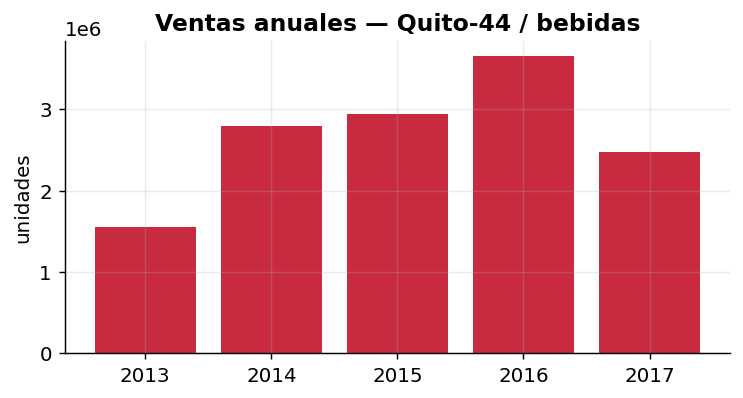
\includegraphics[width=\textwidth]{fig_chart_demo.png}
    \end{column}
  \end{columns}
\end{frame}

% =====================================================================
%  BLOQUE 3 — Prompting
% =====================================================================
\sectionframe{Bloque 3}{Prompting:\\la habilidad clave de hoy}

% F12 — tecnicas
\begin{frame}{El agente es tan bueno como tu pregunta}
  \vspace{8pt}
  \begin{nota}{\small\color{arcaDark}
    Cinco técnicas para un buen prompt:}
  \end{nota}
  \vspace{6pt}
  \begin{enumerate}\setlength\itemsep{4pt}\small
    \item \textbf{Sé específico} --- qué número, qué periodo, qué objeto.
    \item \textbf{Pide el formato} --- "solo el número", "en una tabla", "un gráfico de barras".
    \item \textbf{Da contexto} --- qué representan los datos o las cantidades.
    \item \textbf{Una tarea clara, o divídela} --- si es compleja, enumera los pasos.
    \item \textbf{Pide que muestre el trabajo} --- "muestra el cálculo" para verificar.
  \end{enumerate}
\end{frame}

% F13 — malo vs bueno
\begin{frame}{Mismo objetivo: prompt malo vs. bueno}
  \vspace{6pt}
  \begin{columns}[T]
    \begin{column}{0.48\textwidth}
      \begin{nota}{\footnotesize\color{arcaDark}
        \textcolor{arcaRed}{\faTimes}~\textbf{Malo (vago, pero realista)}\\[3pt]
        \itshape "¿cómo van las ventas?"\\[5pt]
        \upshape Así pregunta un gerente apurado --- pero no dice producto, tienda, año
        ni si quiere unidades o dinero. El agente tiene que \textbf{adivinar}.}
      \end{nota}
    \end{column}
    \begin{column}{0.52\textwidth}
      \begin{idea}{\footnotesize\color{arcaDark}
        \textcolor{codeGreen}{\faCheck}~\textbf{Bueno (específico + formato)}\\[3pt]
        \itshape "¿Cuántas unidades de bebidas vendió Quito-44 en 2016? Dame solo el número."\\[5pt]
        \upshape Dice qué, dónde, cuándo y el formato. Resultado preciso y verificable.}
      \end{idea}
    \end{column}
  \end{columns}
  \vspace{8pt}
  \begin{center}{\small\color{arcaDark}\bfseries
  La diferencia no fue el agente, fue \textbf{el prompt}. Mismo modelo, mejor resultado.}\end{center}
\end{frame}

% =====================================================================
%  BLOQUE 4 — Herramientas + Gradio
% =====================================================================
\sectionframe{Bloque 4}{Más poder:\\herramientas y una app}

% F14 — herramientas
\begin{frame}[fragile]{Darle herramientas al agente}
  \vspace{2pt}
  {\footnotesize Además de escribir código, el agente puede usar \textbf{herramientas
  listas}. smolagents trae varias; una útil es la \textbf{búsqueda web}. Tú no la
  programas: solo la enchufas en \texttt{tools=[...]}.}
  \vspace{6pt}
  \begin{pyblock}
from smolagents import WebSearchTool

agente_web = CodeAgent(tools=[WebSearchTool()], model=modelo)
agente_web.run("Busca el precio actual del azúcar y calcula el costo de 200 kg.")
  \end{pyblock}
  \vspace{4pt}
  \begin{nota}{\footnotesize\color{arcaDark}
    El agente decide cuándo \textbf{buscar} y cuándo \textbf{calcular}. Otras tools:
    leer páginas web, ejecutar Python, transcribir audio --- y conectarse a sistemas
    externos vía el estándar \textbf{MCP}.}
  \end{nota}
\end{frame}

% F15 — Gradio
\begin{frame}[fragile]{Tu agente como app web: Gradio}
  \vspace{4pt}
  \begin{pyblock}
from smolagents import GradioUI
GradioUI(agente).launch(share=True)   # da un link público (en Colab)
  \end{pyblock}
  \vspace{4pt}
  \begin{nota}{\footnotesize\color{arcaDark}
    \texttt{GradioUI} arma un \textbf{chat web} en una línea; \texttt{share=True} da un link
    público temporal.}
  \end{nota}
  \vspace{4pt}
  \begin{idea}{\footnotesize\color{arcaDark}\bfseries
    Ese link se apaga al cerrar el notebook. Para algo \emph{permanente} $\to$ producción real.}
  \end{idea}
\end{frame}

% =====================================================================
%  BLOQUE 5 — Producción / nube / Railway / Open WebUI
% =====================================================================
\sectionframe{Bloque 5}{Del notebook a producción:\\la nube, Railway y tu propia app}

% F16 — Colab se queda corto
\begin{frame}{¿Por qué Colab no basta?}
  \vspace{8pt}
  \begin{center}
  \begin{tikzpicture}[font=\footnotesize, node distance=0.4cm and 1.6cm]
    \node[boxA, text width=4.0cm, align=left] (c)
      {\textbf{Colab}\\\scriptsize se apaga al cerrar\\\scriptsize sin URL permanente\\\scriptsize no recibe peticiones\\\scriptsize solo tú lo usas};
    \node[boxGreen, right=of c, text width=4.0cm, align=left] (p)
      {\textbf{Producción}\\\scriptsize corre 24/7\\\scriptsize URL fija propia\\\scriptsize accesible por tu equipo\\\scriptsize escalable};
    \draw[arrowR] (c)--(p);
  \end{tikzpicture}
  \end{center}
  \vspace{12pt}
  \begin{nota}{\small\color{arcaDark}
    Un asistente real tiene que estar \textbf{disponible siempre} para que tu equipo lo
    use. El notebook es genial para construir y probar, no para que viva ahí.}
  \end{nota}
\end{frame}

% F17 — qué es la nube
\begin{frame}{¿Qué es "la nube"?}
  \vspace{8pt}
  \begin{center}
  \begin{tikzpicture}[font=\footnotesize, node distance=1.2cm]
    \node[boxA, text width=4.2cm, align=center] (a)
      {\textbf{Antes}\\compras y administras\\tu propio servidor físico};
    \node[boxRed, right=of a, text width=4.6cm, align=center] (b)
      {\textbf{La nube}\\alquilas cómputo de otra empresa;\\pagas solo lo que usas};
    \draw[arrowR] (a)--(b);
  \end{tikzpicture}
  \end{center}
  \vspace{12pt}
  \begin{nota}{\small\color{arcaDark}
    Las grandes nubes: \textbf{AWS, Google Cloud, Azure}. Encima de ellas hay
    plataformas más simples para desplegar apps sin pelear con servidores --- una de
    esas es \textbf{Railway}.}
  \end{nota}
\end{frame}

% F18 — qué es Railway
\begin{frame}{¿Qué es Railway?}
  \vspace{8pt}
  \begin{center}
  \begin{tikzpicture}[font=\scriptsize, node distance=0.7cm]
    \node[boxA, text width=2.4cm, align=center] (code) {tu código};
    \node[boxRed, right=of code, text width=2.6cm, align=center] (rail) {Railway\\lo empaqueta\\y lo corre};
    \node[boxGreen, right=of rail, text width=2.8cm, align=center] (url) {URL pública\\funcionando 24/7};
    \draw[arrowR] (code)--(rail); \draw[arrowR] (rail)--(url);
  \end{tikzpicture}
  \end{center}
  \vspace{12pt}
  \begin{nota}{\small\color{arcaDark}
    Le das tu código, te da una dirección web con tu app corriendo. No administras
    servidores. Alternativas parecidas: \textbf{HF Spaces} (gratis, ideal para Gradio),
    Render, Fly.io.}
  \end{nota}
\end{frame}

% F19 — tu propia app, tu propia URL
\begin{frame}{Tu propia app, con tu propia URL}
  \vspace{8pt}
  \begin{center}
  \begin{tikzpicture}[font=\footnotesize, node distance=1.0cm]
    \node[boxRed, text width=4.4cm, align=center, minimum height=1.7cm] (a)
      {\textbf{Es TUYA}\\[3pt]\scriptsize tu propia copia de la app:\\tus datos, tu configuración,\\la controlas tú};
    \node[boxGreen, right=of a, text width=4.9cm, align=center, minimum height=1.7cm] (b)
      {\textbf{Tu propia URL}\\[3pt]\scriptsize una dirección web única\\(\texttt{mi-asistente.up.railway.app})\\que abres y compartes};
  \end{tikzpicture}
  \end{center}
  \vspace{12pt}
  \begin{nota}{\small\color{arcaDark}
    No es una cuenta compartida ni el demo de otro: es \textbf{tu instancia} viviendo en la
    nube, con una \textbf{dirección propia} que tu equipo abre desde cualquier lugar ---
    igual que cualquier sitio web.}
  \end{nota}
\end{frame}

% F20 — manos a la obra: despliegue simple
\begin{frame}{Manos a la obra: tu primera app en producción}
  \vspace{6pt}
  \begin{center}
  \begin{tikzpicture}[font=\scriptsize, node distance=0.5cm]
    \node[boxOrange, text width=2.8cm, align=center, minimum height=1.1cm] (s1) {1. Crea tu cuenta\\en Railway};
    \node[boxBlue, right=of s1, text width=2.8cm, align=center, minimum height=1.1cm] (s2) {2. Despliega un\\template (1 clic)};
    \node[boxGreen, right=of s2, text width=2.8cm, align=center, minimum height=1.1cm] (s3) {3. Espera el\\build};
    \node[boxRed, right=of s3, text width=2.8cm, align=center, minimum height=1.1cm] (s4) {4. Abre TU\\URL pública};
    \draw[arrowD] (s1)--(s2); \draw[arrowD] (s2)--(s3); \draw[arrowD] (s3)--(s4);
  \end{tikzpicture}
  \end{center}
  \vspace{8pt}
  \begin{nota}{\small\color{arcaDark}
    No importa qué app sea: el objetivo es vivir el flujo \textbf{cuenta $\to$ desplegar
    $\to$ tu URL} y ver algo \textbf{tuyo} corriendo en la nube, accesible para cualquiera.}
  \end{nota}
  \vspace{5pt}
  \begin{idea}{\footnotesize\color{arcaDark}\bfseries
    El mismo flujo sirve para subir tu propio agente cuando quieras algo permanente.}
  \end{idea}
\end{frame}

% =====================================================================
%  BLOQUE 6 — Peligros
% =====================================================================
\sectionframe{Bloque 6}{Peligros y cuándo NO\\usar un agente}

% F21 — error en cascada
\begin{frame}{El límite que nadie cuenta: error en cascada}
  \vspace{12pt}
  \begin{center}
  \begin{tikzpicture}
    \node[boxA, text width=11cm, align=center, minimum height=1.3cm] {
      \normalsize Si cada paso acierta el \textcolor{arcaRed}{\textbf{85\%}}
      \;$\Rightarrow$\; 10 pasos: $0.85^{10} \approx$ \textcolor{arcaRed}{\textbf{20\%}}};
  \end{tikzpicture}
  \end{center}
  \vspace{12pt}
  \begin{idea}{\small\color{arcaDark}\bfseries
    Regla de Anthropic: usa lo más simple que funcione. Si puedes \textbf{dibujar el
    árbol de decisión} de la tarea, no uses un agente --- escribe un flujo fijo. El
    agente es para tareas \textbf{abiertas}.}
  \end{idea}
\end{frame}

% F22 — reglas de oro
\begin{frame}{Reglas de oro}
  \vspace{10pt}
  \begin{itemize}\setlength\itemsep{8pt}
    \item \texttt{max\_steps} y un \textbf{límite de costo}, siempre.
    \item El CodeAgent \textbf{ejecuta código} que el modelo escribió: en producción,
      córrelo en \textbf{sandbox} (E2B, Docker), no abierto.
    \item La \textbf{lista blanca} de imports es tu primera defensa.
    \item Si la tarea es fija y conocida, \textbf{no uses un agente}.
  \end{itemize}
\end{frame}

% =====================================================================
%  CIERRE
% =====================================================================
\sectionframe{Cierre}{Lo que te llevas}

% F23 — recap
\begin{frame}{Lo que te llevas}
  \vspace{6pt}
  \begin{enumerate}\setlength\itemsep{5pt}
    \item Un \textbf{agente} = un LLM en un bucle \emph{pensar $\to$ actuar $\to$ observar} (ReAct).
    \item El \textbf{CodeAgent} actúa escribiendo código. Estructura: modelo +
      \texttt{CodeAgent} + \texttt{run}.
    \item \textbf{El buen prompting es la habilidad clave}: específico + formato + contexto.
    \item Le puedes dar \textbf{herramientas} (búsqueda web) sin programar.
    \item \texttt{GradioUI} lo vuelve app; \textbf{Railway} lo lleva a producción (tu propia URL).
    \item Cuídalo: \texttt{max\_steps}, sandbox, y si la tarea es fija, no uses agente.
  \end{enumerate}
  \vspace{6pt}
  \begin{idea}{\small\color{arcaDark}\bfseries
    La habilidad que cambia: ya no es "saber escribir pandas", es \textbf{saber pedir bien}.}
  \end{idea}
\end{frame}

% F24 — gracias
\begin{frame}[plain, noframenumbering]
  \begin{tikzpicture}[remember picture, overlay]
    \fill[arcaDark] (current page.south west) rectangle (current page.north east);
    \node[anchor=center, text=white, font=\Huge\bfseries] at
      ([yshift=1cm]current page.center) {Gracias};
    \node[anchor=center, text=white!85, font=\Large] at
      ([yshift=-0.2cm]current page.center) {¿Preguntas?};
    \node[anchor=center, text=white!70, font=\small] at
      ([yshift=-1.5cm]current page.center)
      {Clase 37 --- Agentes: el analista que programa por ti};
    \node[anchor=center, text=white!60, font=\scriptsize] at
      ([yshift=-2cm]current page.center)
      {github.com/cmosquerat/arca-diplomado/tree/main/clase-37};
  \end{tikzpicture}
\end{frame}

\end{document}
